\documentclass[11pt,a4paper]{article}
\usepackage[utf8]{inputenc}
\usepackage[spanish,es-tabla]{babel}
\usepackage{amsmath}
\usepackage{amsfonts}
\usepackage{amssymb}
\usepackage{graphicx}
\usepackage{natbib}
\usepackage{lineno}
\usepackage{ragged2e}
\usepackage{multicol}
\setlength\columnsep{38pt}
\usepackage{enumerate} 
\usepackage[left=2.8cm,top=2.3cm,right=2.8cm,bottom=2.3cm]{geometry} 
\usepackage{fancyhdr}
\usepackage{url}


\begin{document}
		
		\begin{center}
			\huge \textbf{Aprendizaje Supervisado y No Supervisado} 
		\end{center}
		
		\begin{center}
			
\includegraphics[scale=0.50]{./Imagenes/logo}
		\end{center}
		
		\begin{multicols}{2}
			\small
			\begin{center}
				Marlon Villegas Arando\\
				2015053890\\
				UPT – Ingeniería de Sistemas\\
				EPIS\\
				Tacna, Perú\\
				
				\vspace{\baselineskip}
				Lisbeth Espinoza Caso\\
				2011040667\\
				UPT – Ingeniería de Sistemas\\  
				EPIS\\	
				Tacna, Perú\\                 

			\end{center}
			\normalsize			
		\end{multicols}
		\vspace{\baselineskip}

		\textbf{\textit{\large Resumen}}\rule[1.5mm]{5mm}{0.1mm}	\vspace{\baselineskip}
		
		\\La inteligencia, en pleno siglo XXI, trasciende las fronteras de la mente. Mucho escuchamos decir que ahora los computadores son más inteligentes que los cerebros y que pronto los robots sustituirán a los humanos para pasar a dominar el mundo.\\
		
        \\Está muy arraigada la creencia de que por más inteligente que pueda ser un computador, nunca podrá tener la capacidad de pensar. Sin ánimos de fatalismo, el aprendizaje automático ha revolucionado de forma decisiva el campo de la computación, facilitando la realización de todo tipo de tareas de forma digital y no manual.\\ 
        
        \\El aprendizaje automático, también conocido en inglés como machine learning, es un campo de la computación que lleva a otro nivel a la inteligencia artificial: hace que las computadoras aprendan a pensar.\\
        
        \\No tan literal. Los computadores no desarrollaron un cerebro y ahora tienen emociones. Simplemente el machine learning desarrolla algoritmos que hacen que las máquinas puedan aprender por su cuenta y responder a determinadas preguntas con bastante certeza. Para desarrollar estos algoritmos, existen dos modalidades: aprendizaje supervisado y no supervisado.\\
		
		\newpage
		
		\textbf{\textit{\large Abstract}}\rule[1.5mm]{5mm}{0.1mm} 		
		\textit{	
		 }\vspace{\baselineskip}
		 \\The intelligence, in the 21st century, transcends the frontiers of the mind. We hear a lot to say that computers are now smarter than brains and that soon robots will replace humans to dominate the world.\\
		 
		 \\The belief that as intelligent as a computer may be, it can never have the ability to think is deeply rooted. Without the spirit of fatalism, machine learning has revolutionized the field of computing decisively, making it easier to perform all kinds of tasks digitally and not manually.\\
		 
		 \\Machine learning, also known in English as machine learning, is a field of computing that takes artificial intelligence to another level: it makes computers learn to think\\
		 
		 \\Not so literal. Computers did not develop a brain and now have emotions. Machine learning simply develops algorithms that allow machines to learn on their own and answer certain questions with certainty. To develop these algorithms, there are two modalities: supervised and unsupervised learning.\\
				
		\vspace{\baselineskip}
					
		\rule{167mm}{0.1mm}
		
		\vspace{\baselineskip}
		
		\section{Introduccion}
		
		El aprendizaje automático o machine learning se encuadra como una disciplina de la inteligencia artificial.\\

        El principal objetivo que busca es crear sistemas que sean capaces de aprender automáticamente, es decir que sean capaces de encontrar patrones complejos en grandes conjuntos de datos por si solos.\\

        Los algoritmos de machine learning se suelen clasificar en dos grupos, por un lado se encuentran los algoritmos supervisados que aplican lo que se ha aprendido con los datos históricos para sacar conclusiones sobre nuevos datos y por otro lado se encuentran los algoritmos no supervisados pueden extraer inferencias de conjuntos de datos, aunque existen otros tipos como aprendizaje semi-supervisado, aprendizaje por refuerzo, aprendizaje multi-tarea y transducción.\\
		
		\begin{center}
		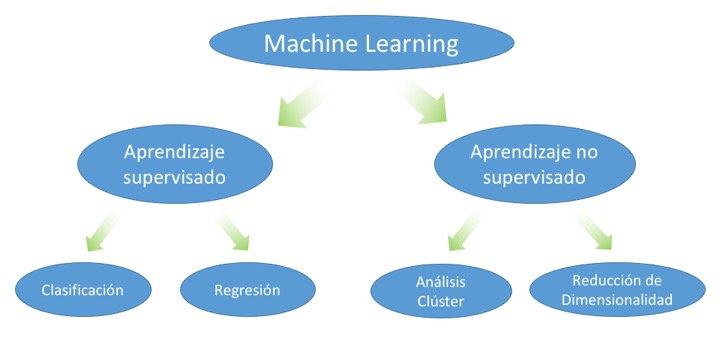
\includegraphics[scale=0.5]{./Imagenes/MachineLearning}
		\end{center}
		
		\section{Aprendizaje Supervisado}
		
			El aprendizaje supervisado es el más común utilizado entre los dos , incluye algoritmos tales como regresión lineal y logístico, clasificación de clases múltiples y máquinas de vectores de soporte.\\

            El aprendizaje supervisado se llama así porque el desarrollador actúa como una guía para enseñar al algoritmo las conclusiones a las que debe llegar, es decir la salida del algoritmo ya es conocida. Es similar a la forma en que un niño podría aprender de un maestro.\\

            Requiere que los posibles resultados del algoritmo ya sean conocidos y que los datos utilizados para entrenar el algoritmo ya estén etiquetados con las respuestas correctas. Por ejemplo, un algoritmo de clasificación aprenderá a identificar animales después de haber sido entrenados en un conjunto de datos de imágenes que están apropiadamente etiquetados con las especies del animal y algunas características de identificación.\\
            
            \begin{center}
		    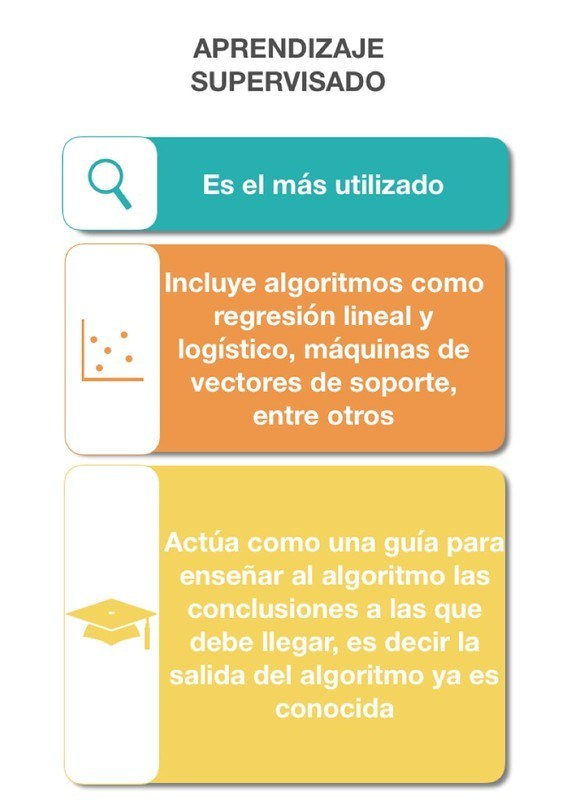
\includegraphics[scale=1.0]{./Imagenes/AprendisajeSupervisado}
		    \end{center}
			
			\subsection{Funciones y Tipos}
			\\La primera modalidad de aprendizaje que tiene el machine learning es la de aprendizaje supervisado. Usándola, se entrena al algoritmo otorgándole las preguntas, denominadas características, y las respuestas, denominadas etiquetas. Esto se hace con la finalidad de que el algoritmo las combine y pueda hacer predicciones.\\
            
            \\Existen, a su vez, dos tipos de aprendizaje supervisado:\\
		
			\begin{enumerate}[A.]
			
			\item Regresión:
			
			    Tiene como resultado un número específico. Si las etiquetas suelen ser un valor numérico, mediante las variables de las características, se pueden obtener dígitos como dato resultante.\\
			
			    \begin{center}	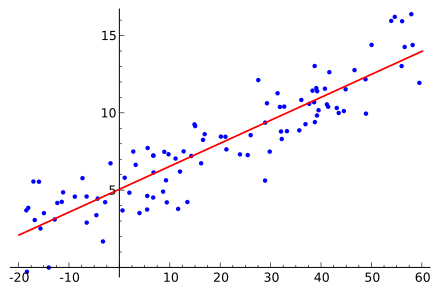
\includegraphics[scale=0.5]{./Imagenes/regresion}
    			\end{center}
			
			    \\Donde se predice un valor real basado en entradas pasadas. Estos algoritmos se usan para predecir valores de salida basados en algunas características de entrada obtenidas de los datos. A esto, el algoritmo construye un modelo basado en las características y los valores de salida de los datos de entrenamiento y este modelo se usa para predecir los valores para nuevos datos. Los valores de salida en este caso son continuos y no discretos.\\

                \\Algunos ejemplos de este algoritmo son: predecir los precios de la vivienda, predecir las cantidades de compra, predecir la cantidad de ingresos se genera a partir de una nueva campaña de marketing.\\
                
                \\Los tipos de algoritmos de regresión incluyen:\\
                
                \begin{itemize}
			    \item Regresión lineal
			    \item Regresión polinomeal
			    \item Vectores de soporte regresión
			    \item Arboles de decisión regresión
			    \item Bosques aleatorios regresión
		        \end{itemize}
                
                \begin{center}
		        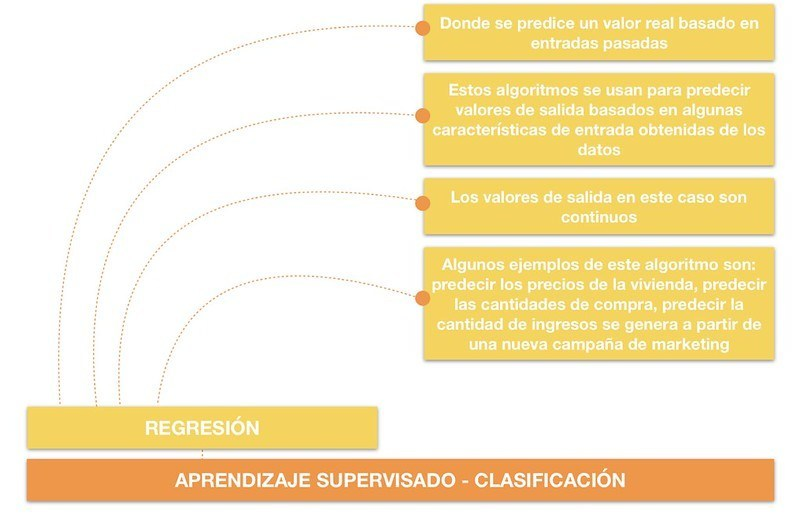
\includegraphics[scale=1.0]{./Imagenes/AprendSuperRegresion}
		        \end{center}

    		\item Clasificación: 
    		    
    		    \\En este tipo, el algoritmo encuentra diferentes patrones y tiene por objetivo clasificar los elementos en diferentes grupos.\\
			
    			\begin{center}	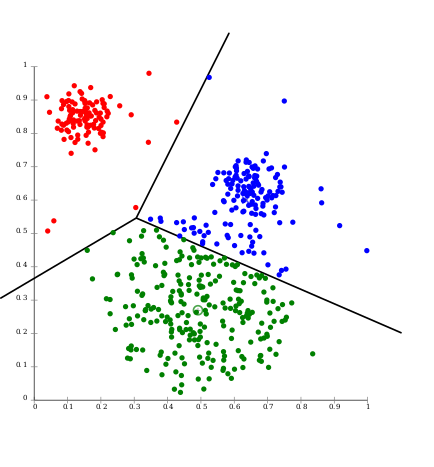
\includegraphics[scale=0.5]{./Imagenes/clasificacion}
    			\end{center}
			
			    \\El algoritmo no está en capacidad de determinar a qué grupo pertenece un valor o cuál es el resultado de una operación. Solamente logra relacionar características con etiquetas y así obtener un resultado.\\
			    
			    \\El algoritmo intenta etiquetar cada ejemplo eligiendo entre dos o más clases diferentes. Estos algoritmos crean modelos predictivos a partir de datos de capacitación que tienen características y etiquetas de clase.\\
			    
			    \\Estos modelos predictivos, a su vez usan las características aprendidas de los datos de capacitación sobre datos nuevos, no vistos previamente, para predecir sus etiquetas de clase. Elegir entre dos clases se denomina clasificación binaria, como predecir si alguien incumplirá un préstamo. Elegir entre más de dos clases se denomina clasificación multiclase.\\

                \\Algunos ejemplos de este algoritmo son: predecir si un cliente va a cancelar o no su tarjeta de crédito, predecir si un alumno pasará o no una clase.\\

                \\Los tipos de algoritmos de clasificación incluyen:\\

                \begin{itemize}
			    \item Regresión logística
			    \item Vecinos más cercanos
			    \item Máquinas de vectores de soportes
			    \item Arboles de decisión clasificación
			    \item Bosques aleatorios clasificación
		        \end{itemize}
                
                \begin{center}
		        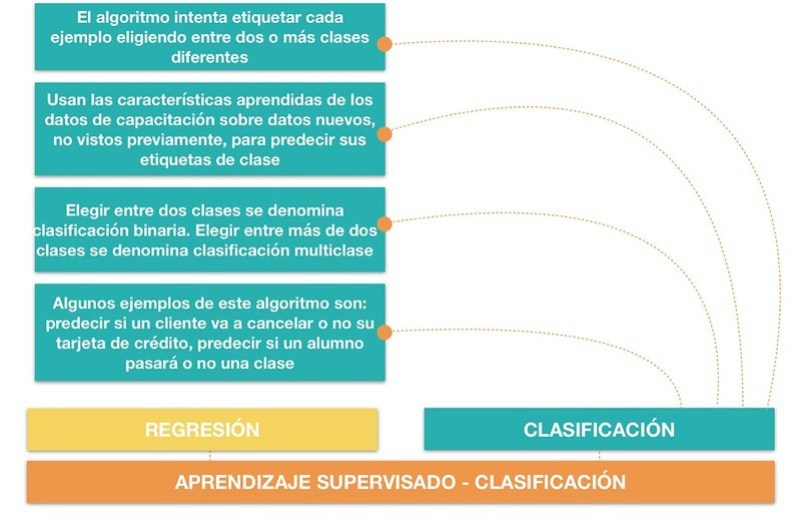
\includegraphics[scale=1.0]{./Imagenes/AprendSuperClasificacion}
		        \end{center}
			
			\end{enumerate}
			
		    \\En el aprendizaje supervisado, los algoritmos trabajan con datos “etiquetados” (labeled data), intentado encontrar una función que, dadas las variables de entrada (input data), les asigne la etiqueta de salida adecuada. El algoritmo se entrena con un “histórico” de datos y así “aprende” a asignar la etiqueta de salida adecuada a un nuevo valor, es decir, predice el valor da salida.\\

            \\Por ejemplo, un detector de spam, analiza el histórico de mensajes, viendo qué función puede representar, según los parámetros de entrada que se definan (el remitente, si el destinatario es individual o parte de una lista, si el asunto contiene determinados términos etc), la asignación de la etiqueta “spam” o “no es spam”. Una vez definida esta función, al introducir un nuevo mensaje no etiquetado, el algoritmo es capaz de asignarle la etiqueta correcta.\\

            \\El aprendizaje supervisado se suele usar en problemas de clasificación, como identificación de dígitos, diagnósticos, o detección de fraude de identidad.  También se usa en problemas de regresión, como predicciones meteorológicas, de expectativa de vida, de crecimiento etc. Estos dos tipos principales de aprendizaje supervisado, clasificación y regresión, se distinguen por el tipo de variable objetivo. En los casos de clasificación, es de tipo categórico, mientras que, en los casos de regresión, la variable objetivo es de tipo numérico.\\
            
            \subsection{Aprendizaje Supervisado en el Machine Learning}
            
            \\El objetivo básico de Machine Learning es utilizar computadoras para obtener información, sin que se indique explícitamente que lo haga. En la mayoría de los casos esto implica utilizar un conjunto de resultados históricos para hacer predicciones sobre los resultados futuros.\\ 
            
            \\Esto se vuelve útil cuando se quiere automatizar las percepciones sobre conjuntos de datos de gran tamaño, lo que sería demasiado difícil de realizar para un ser humano de manera recurrente.\\
            
            \begin{center}	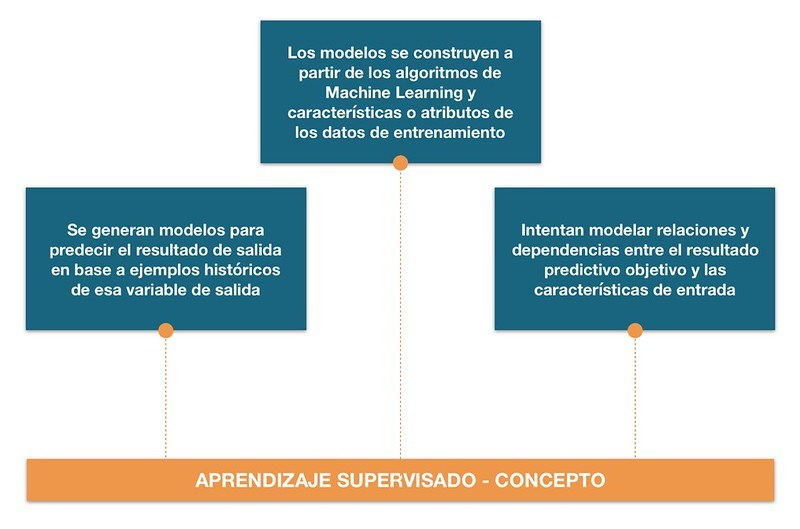
\includegraphics[scale=1.0]{./Imagenes/AprendizajeSupervisadoConcepto}
    		\end{center}
    		
    		\\Por su parte, el aprendizaje supervisado se refiere al subconjunto de Machine Learning donde se generan modelos para predecir el resultado de salida en base a ejemplos históricos de esa variable de salida.\\ 
    		
    		\\Los modelos se construyen a partir de los algoritmos de Machine Learning y características o atributos de los datos de entrenamiento para que podamos predecir el valor utilizando otros valores obtenidos a partir de datos de entrada.\\

            \\Los algoritmos de aprendizaje supervisado intentan modelar relaciones y dependencias entre el resultado predictivo objetivo y las características de entrada para que podamos predecir los valores de salida para datos nuevos en función de las relaciones que aprendió de los conjuntos de datos anteriores.\\
            
            \subsection{Importancia del aprendizaje supervisado}
            
            \\El aprendizaje supervisado proporciona una ruta directa para convertir datos en información real y procesable. Al utilizar los datos como un recurso, les permite a las organizaciones comprender y prevenir los resultados no deseados o impulsar los resultados deseados para lo que sea que estén tratando de predecir.\\

            \\Por ejemplo, pueden decirle a una empresa que los clientes presentan un alto riesgo de agitación, la compañía puede llegar a ese cliente en particular con comunicaciones dirigidas y ofertas promocionales, lo que reduce su predisposición al abandono.\\

            \\Este aprendizaje es uno de los motores más potentes que permite que los sistemas de inteligencia artificial tomen decisiones empresariales de forma más rápida y precisa que los humanos.\\

            \\Sin embargo, la implementación exitosa de algoritmos de aprendizaje supervisado ha requerido gran cantidad de tiempo y la experiencia técnica de equipos especializados con el fin de construir, escalar y desplegar modelos predictivos precisos. Además, dado que los modelos de aprendizaje supervisado hacen predicciones del mundo real basado en los datos del pasado, los modelos deben ser reconstruidos periódicamente con el fin de mantener sus predicciones sin que se conviertan en obsoletas ya que en ocasiones el comportamiento de los datos puede cambiar.\\
            
            \begin{center}	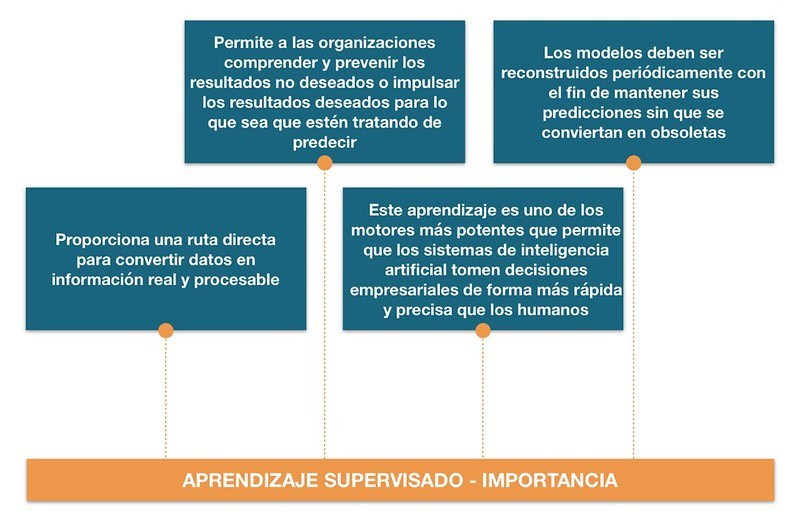
\includegraphics[scale=1.0]{./Imagenes/AprendSuperImportancia}
    		\end{center}
    		
    		\\En conclusión, el aprendizaje supervisado aprende de datos etiquetados, es decir, los datos del cual conoce la variable resultado, y hace predicciones para ese resultado en nuevos conjuntos de datos. Es importante tener en cuenta que solo funciona si su conjunto de datos históricos contiene valores reales para el resultado que intenta predecir.\\

	        \subsection{Algoritmos de Clasificación}
	        
	        \begin{enumerate}[A.]
		
			\item \textbf{Regresión Logística:}
			
			\\Uno de los principales problemas en la clasificación ocurre cuando el algoritmo nunca converge en la actualización de los pesos mientras está siendo entrenado.\\
            
            \\Esto ocurre cuando las clases no son perfectamente separables linealmente. Por tanto, para tratar con problemas de clasificación binaria la regresión logística es uno de los algoritmos más usados.\\
            
            \\La regresión logística es un algoritmo de clasificación (a pesar de su nombre) simple, pero potente . Funciona muy bien en clases linealmente separables y se puede extender a clasificación multiclase , a través de la técnica OvR.\\
			
			\item \textbf{Máquinas de Vector Soporte (SVM):}
			
			\\Este algoritmo puede ser considerado una extensión del algoritmo “perceptron”. En SVM el objetivo de la optimización es establecer una línea de decisión que separe las clases maximizando el margen entre esta línea y los puntos de muestra cercanos a este hiperplano. Estos puntos se llaman vectores soporte.\\
			
			\begin{center}
		    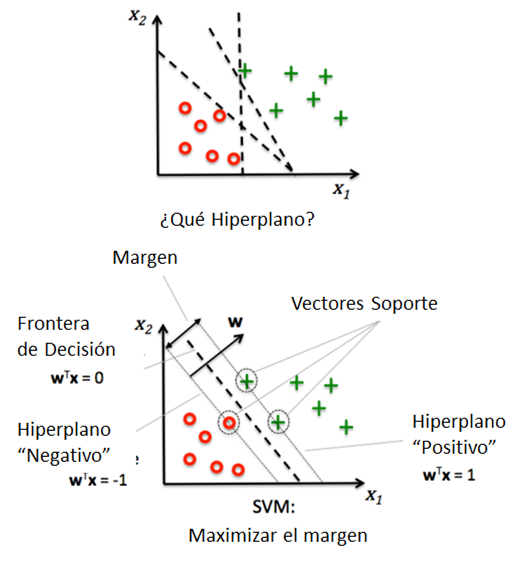
\includegraphics[scale=0.7]{./Imagenes/SVM}
		    \end{center}
\item \textbf{Algoritmos de Árbol de Decisión:}
			
			\\Los algoritmos de árbol de decisión desglosan el conjunto de datos mediante la formulación de preguntas hasta conseguir el fragmento de datos adecuado para hacer una predicción.\\
            
            \\Para verlo de una manera gráfica, consideremos un ejemplo de un árbol de decisión para determinar si es adecuado prestarle el automóvil a alguien:\\
			
			\begin{center}
		    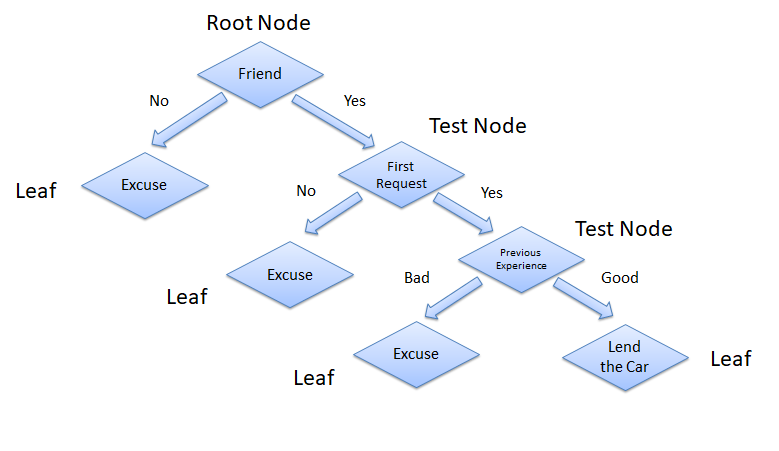
\includegraphics[scale=0.5]{./Imagenes/ArbolDeDecision}
		    \end{center}
			
			\\Basado en las características de los datos de entrenamiento, el árbol de decisión “aprende” una serie de factores para inferir las etiquetas de clase de los ejemplos.\\

            \\El nodo de comienzo es la raíz del árbol, y el algoritmo dividirá de forma iterativa el conjunto de datos en la característica que contenga la máxima ganancia de información, hasta que los nodos finales (hojas) sean puros.\\

            \item \textbf{Bosques Aleatorios (Random Forests):}
            
			\\Si tenemos un conjunto de datos con muchas características (columnas), el algoritmo del árbol de decisión tiende a sobreajustar, añadiendo complejidad al modelo y el proceso de aprendizaje.\\
            
            \\Podemos solventar este punto seleccionando cada columna de forma aleatoria y realizando árboles de decisión para cada conjunto de columnas.\\
			
			\begin{center}
		    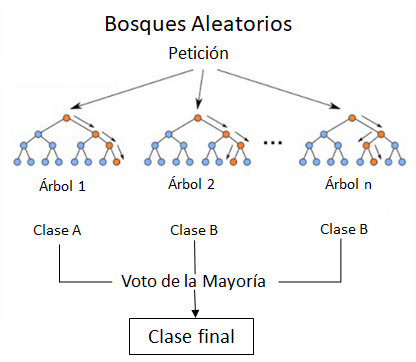
\includegraphics[scale=0.7]{./Imagenes/BosqueAleatorios}
		    \end{center}
			
			\\De esta forma, se desarrolla un algoritmo de agrupación de aprendizaje que combinará una serie de modelos más débiles para crear otro más robusto.\\
            
            \\El algoritmo realizará los siguientes pasos:\\

            \begin{itemize}
			    \item Diseñar una muestra de arranque de tamaño n.
			    \item Desarrollar un árbol de decisión desde la muestra de arranque.
			    \item En cada nodo habrá características seleccionadas aleatoriamente sin reemplazamiento y el nodo se cortará maximizando la ganancia de información.
			    \item El proceso previo se repetirá K veces.
			    \item Agregar la predicción hecha para cada árbol, asignando la etiqueta de clase por votación mayoritaria.
		    \end{itemize}

            \\La principal ventaja de este método es que normalmente no necesitaremos podar el bosque aleatorio (ya que el modelo es muy resistente al ruido). Sin embargo, es mucho menos interpretable que los árboles de decisión.\\

            \\El único hiperparámetro que necesitaremos ajustar es el número de árboles K. Normalmente, cuanto más grande es K , mejor se comportará el modelo, pero esto incrementará drásticamente el esfuerzo de computación (y por tanto, el coste).\\

            \item \textbf{Los K-vecinos Más Cercanos (K Nearest Neighbors or KNN):}
            
            \\Los K-vecinos más cercanos, o KNN, pertenecen a un tipo especial de modelos de machine learning que se llaman frecuentemente “algoritmos perezosos”.\\

            \\Reciben este nombre porque no aprenden cómo discriminar el conjunto de datos con una función optimizada, en su lugar memorizan el conjunto de datos.\\
            
            \\El nombre también se refiere a la clase de algoritmos llamados “no paramétricos”. Estos son algoritmos basados en instancia , que se caracterizan por memorizar el conjunto de datos de entrenamiento, y el apredizaje perezoso es un caso particular de estos algoritmos, asociados con coste computacional cero durante el aprendizaje.\\

             \\El proceso que sigue el algoritmo es:\\
            
            \begin{itemize}
			    \item Escoge el número de k y la distancia.
			    \item Encuentra el k vecino más cercano de la muestra que se pretende clasificar.
			    \item Asigna la etiqueta de clase por votación mayoritaria.
		    \end{itemize}
		    
		    \begin{center}
		    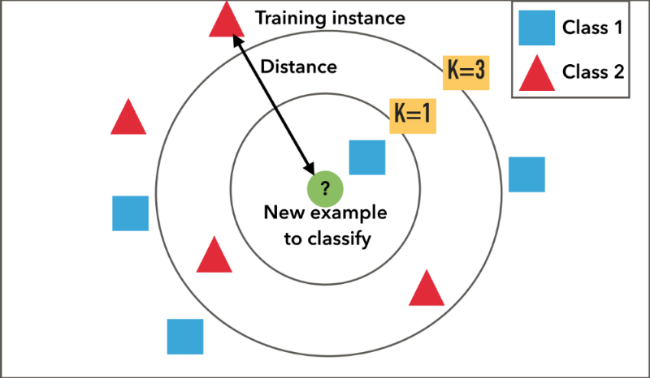
\includegraphics[scale=0.5]{./Imagenes/KNN}
		    \end{center}

            \\El algoritmo encuentra las k muestras que son más cercanas al punto que se quiere clasificar, basando sus predicciones en la distancia métrica.\\

            \\La principal ventaja es que se adapta a los nuevos datos de entrenamiento, al ser un algoritmo basado en la memoria. La desventaja es que el coste computacional se incrementa linealmente con el tamaño de los datos de entrenamiento.\\

			\end{enumerate}
	    
	    \newpage
	    
	    \section{Aprendizaje No Supervisado}
		
		\\El aprendizaje no supervisado está más estrechamente alineado con la inteligencia artificial, ya que la idea de que una computadora pueda aprender a identificar procesos y patrones complejos sin un humano para proporcionar orientación a lo largo del camino. Algunos ejemplos de algoritmos de aprendizaje no supervisado incluyen clustering o agrupamiento, k-means y reglas de asociación.\\

        \\Acá no existe un conjunto de datos de entrenamiento y los resultados son desconocidos. Esencialmente, se entra en el problema de manera ciega y con solo operaciones lógicas impecables para guiarlo, aunque parezca increible, el aprendizaje no supervisado es la capacidad de resolver problemas complejos utilizando solo los datos de entrada y los alogoritmos lógicos, y en ningún momento se tiene datos de referencias.\\
		
		\begin{center}
		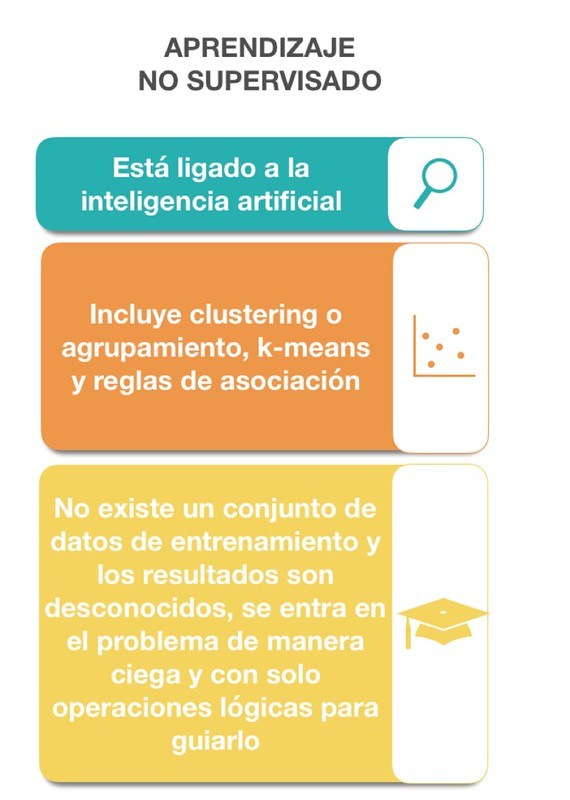
\includegraphics[scale=1.0]{./Imagenes/AprendisajeNoSupervisado}
		\end{center}
		
		\\Un ejemplo muy simple de ambos aprendizaje es que digamos que tenemos una imagen digital que muestra una serie de formas geométricas de colores que debemos unir en grupos según su clasificación y color, este es un problema muy común en las aplicaciones de reconocimiento de imágenes de Machine Learning.\\

        \\Con el aprendizaje supervisado, la solución a este problema es bastante sencillo, simplemente le enseñamos a la computadora que las formas con cuatro lados se conocen como cuadrados  y las formas de tres lados se conocen como triángulos. También le indicamos que si la luz emitida por un pixel registra ciertos valores, lo clasificamos rojo y otro conjunto de valores como azul. De esta forma muy sencilla nuestro algoritmo ha aprendido a agrupar el conjunto de formas geométricas dado.\\
		
		\begin{center}
		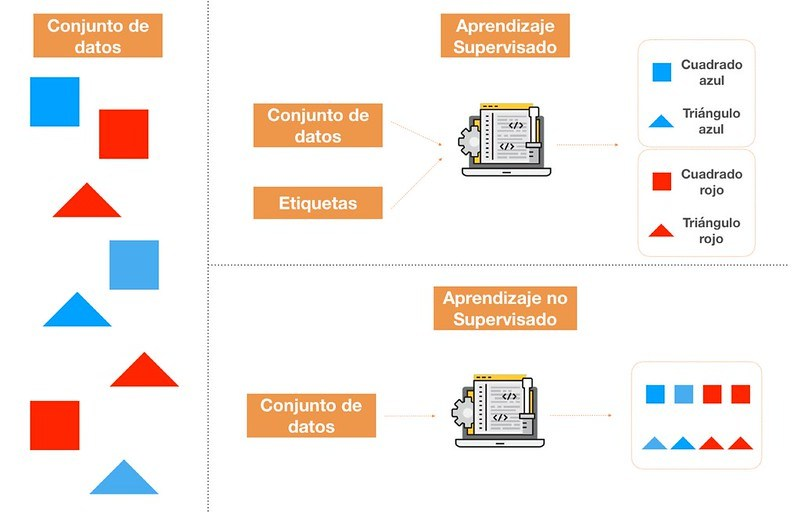
\includegraphics[scale=1.0]{./Imagenes/EjemploAprendizajeNoSupervisado}
		\end{center}
		
		\\Ahora bien con el aprendizaje no supervisado, la solución a este problema se vuelve un poco más complicado. Acá el algoritmo tiene los mismos datos de entrada, imágenes digitales que muestran formas geométricas en diferentes colores y queremos ordenarlos en grupos. Para solucionar este problema, el algoritmo aprende de la información: el problema es de clasificación y que algunas de las formas coinciden con otras, quizás con el mismo número de lados o con marcadores digitales que coinciden con el color.\\
		
		\\El algoritmo no puede saber que el nombre de los objetos es cuadrado o triangulo, pero si reconocerá otros objetos con más o menos las mismas características y los agrupará asignandoles su propia etiqueta. De esta forma el algoritmo ha resulto el problema dado.\\

        \\Tecnicamente no hay respuesta correcta o incorrecta, Machine Learning simplemente aprenderá la verdad objetiva de que ciertas formas pertenecen juntas hasta cierto grado de probabilidad. Obviamente, Machine Learning comete errores pero, como nosotros, su fortaleza radica en su capacidad para aprender de sus errores y hacer estimaciones mejor educadas la próxima vez.\\

        \\La elección de de utilizar un algoritmo de Machine Learning supervisado o no supervisado generalmente depende de factores relacionados con la estructura y el volumen de sus datos y del objetivo del problema en cuestión. Un problema complejo por lo general utilizará ambos tipos de algoritmos para construir modelos de datos predictivos que ayuden a tomar decisiones sobre una variedad de desafíos comerciales.\\
		
		
		
		
		
		
		\newpage
		\section{Diferencias entre el aprendizaje supervisado y el aprendizaje no supervisado}
		
		\\Los estudiantes que se aventuran en el aprendizaje automático han experimentado dificultades para diferenciar el aprendizaje supervisado del aprendizaje no supervisado. Parece que el procedimiento utilizado en ambos métodos de aprendizaje es el mismo, lo que hace que sea difícil diferenciar entre los dos métodos de aprendizaje. Sin embargo, tras el escrutinio y la atención inquebrantable, uno puede entender claramente que existen diferencias significativas entre el aprendizaje supervisado y el no supervisado.\\
		
	    \begin{center}	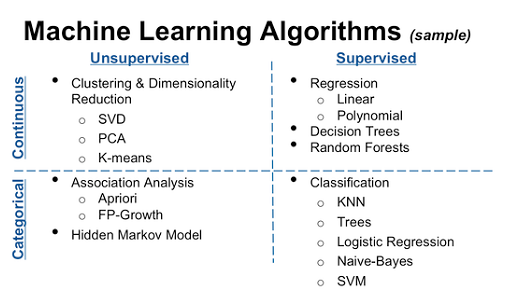
\includegraphics[scale=0.9]{./Imagenes/Diferencias}	
		\end{center}
	
		\subsection{Datos de entrada en aprendizaje supervisado y aprendizaje no supervisado}
		
		\\La principal diferencia entre el aprendizaje supervisado y el aprendizaje no supervisado es la información utilizada en cualquiera de los métodos de aprendizaje automático. Vale la pena señalar que ambos métodos de aprendizaje automático requieren datos, que analizarán para producir ciertas funciones o grupos de datos.\\ 
		\\Sin embargo, los datos de entrada utilizados en el aprendizaje supervisado son bien conocidos y están etiquetados. Esto significa que la máquina solo tiene la función de determinar los patrones ocultos de los datos ya etiquetados. Sin embargo, los datos utilizados en el aprendizaje no supervisado no se conocen ni etiquetan.\\
		\\El trabajo de la máquina consiste en categorizar y etiquetar los datos brutos antes de determinar los patrones y funciones ocultos de los datos de entrada.\\
		
		\subsection{Complejidad Computacional en Aprendizaje Supervisado y Aprendizaje No Supervisado}
		
		\\El aprendizaje automático es un asunto complejo y cualquier persona involucrada debe estar preparada para la tarea que le espera. Una de las diferencias sobresalientes entre el aprendizaje supervisado y el aprendizaje no supervisado es la complejidad computacional. \\
		\\Se dice que el aprendizaje supervisado es un método complejo de aprendizaje, mientras que el método de aprendizaje no supervisado es menos complejo. Una de las razones por las que el asunto del aprendizaje supervisado es el hecho de que uno tiene que entender y etiquetar las entradas mientras se está en el aprendizaje no supervisado, no se requiere que uno entienda y etiquete las entradas. \\
		\\Esto explica por qué muchas personas han estado prefiriendo el aprendizaje no supervisado en comparación con el método supervisado de aprendizaje automático.\\

        \subsection{Precisión de los resultados del aprendizaje supervisado y el aprendizaje no supervisado}
		
		\\La otra diferencia que prevalece entre el aprendizaje supervisado y el aprendizaje no supervisado es la precisión de los resultados producidos después de cada ciclo de análisis de la máquina. \\
		\\Todos los resultados generados por el método supervisado de aprendizaje automático son más precisos y confiables en comparación con los resultados generados por el método de aprendizaje automático no supervisado. Uno de los factores que explica por qué el método supervisado de aprendizaje automático produce resultados precisos y confiables es porque los datos de entrada son bien conocidos y etiquetados, lo que significa que la máquina solo analizará los patrones ocultos. \\
		\\Esto es diferente al método de aprendizaje no supervisado donde la máquina tiene que definir y etiquetar los datos de entrada antes de determinar los patrones y funciones ocultos.\\
		
		\subsection{Número de clases en Aprendizaje Supervisado y Aprendizaje No Supervisado}
		
		\\También vale la pena señalar que hay una diferencia significativa cuando se trata de la cantidad de clases. Vale la pena señalar que todas las clases utilizadas en el aprendizaje supervisado son conocidas, lo que significa que también es probable que se conozcan las respuestas en el análisis. \\
		\\El único objetivo del aprendizaje supervisado es, por lo tanto, determinar el grupo desconocido. Sin embargo, no hay conocimiento previo en el método de aprendizaje automático no supervisado. \\
		\\Además, se desconoce el número de clases, lo que significa claramente que no se conoce ninguna información y que los resultados se generan después de que no se puede determinar el análisis.\\
		\\Además, las personas involucradas en el método de aprendizaje no supervisado no conocen ninguna información relacionada con los datos en bruto y los resultados esperados.\\
		
		\subsection{Aprendizaje en tiempo real en aprendizaje supervisado y aprendizaje no supervisado}
		
		\\Entre otras diferencias, existe el tiempo después del cual cada método de aprendizaje tiene lugar. \\
		\\Es importante resaltar que el método de aprendizaje supervisado se lleva a cabo fuera de línea mientras que el método de aprendizaje no supervisado se lleva a cabo en tiempo real. \\
		\\Las personas involucradas en la preparación y etiquetado de los datos de entrada lo hacen fuera de línea mientras que el análisis del patrón oculto se realiza en línea, lo que niega a las personas involucradas en el aprendizaje automático la oportunidad de interactuar con la máquina mientras analiza los datos discretos.\\ 
		\\Sin embargo, el método de aprendizaje automático no supervisado se lleva a cabo en tiempo real de manera que todos los datos de entrada se analizan y etiquetan en presencia de los alumnos, lo que les ayuda a comprender los diferentes métodos de aprendizaje y clasificación de los datos en bruto.\\
		\\El análisis de datos en tiempo real sigue siendo el mérito más importante del método de aprendizaje no supervisado.\\
		
		\begin{center}
		\caption{TABLA QUE MUESTRA LAS DIFERENCIAS ENTRE EL APRENDIZAJE SUPERVISADO Y EL APRENDIZAJE NO SUPERVISADO}
		\end{center}
		
		\begin{center}	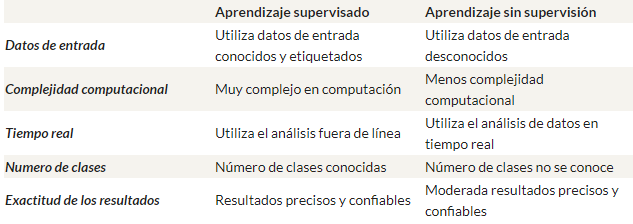
\includegraphics[scale=0.9]{./Imagenes/CuadroDiferencia}	
		\end{center}	
			
		
		\newpage
		\section{Conclusiones}
		\\La minería de datos se está convirtiendo en un aspecto esencial en el mundo empresarial actual debido al aumento de los datos brutos que las organizaciones necesitan analizar y procesar para que puedan tomar decisiones sólidas y confiables.\\
        
        \\Esto explica por qué la necesidad de aprendizaje automático está creciendo y, por lo tanto, requiere personas con suficiente conocimiento tanto del aprendizaje automático supervisado como del aprendizaje automático no supervisado.\\

        \\Vale la pena entender que cada método de aprendizaje ofrece sus propias ventajas y desventajas. Esto significa que uno tiene que estar familiarizado con ambos métodos de aprendizaje automático antes de determinar qué método utilizará para analizar los datos.\\
	
	    \\El aprendizaje supervisado es uno de los métodos asociados con el aprendizaje automático que implica la asignación de datos etiquetados para que se pueda deducir un determinado patrón o función a partir de esos datos. Vale la pena señalar que el aprendizaje supervisado implica la asignación de un objeto de entrada, un vector, mientras que, al mismo tiempo, anticipa el valor de salida más deseado, que se conoce principalmente como la señal de supervisión. La propiedad final del aprendizaje supervisado es que los datos de entrada son conocidos y etiquetados adecuadamente.\\
	    
	    \\El aprendizaje no supervisado es el segundo método de algoritmo de aprendizaje automático donde las inferencias se obtienen de datos de entrada sin etiqueta. El objetivo del aprendizaje no supervisado es determinar los patrones ocultos o la agrupación en datos de datos no etiquetados. Se usa principalmente en el análisis de datos exploratorios. Uno de los caracteres definitorios del aprendizaje no supervisado es que tanto la entrada como la salida no se conocen.\\
			
	    
\end{document}		
